\begin{figure}[htbp]
\centering
% Encoder colors (reuse from Nature CNN)
\definecolor{encfade}{HTML}{B8D2E6}
% SPR-specific component color
\definecolor{sprcomp}{HTML}{C2D4A8}
\definecolor{sprfade}{HTML}{D8E4CC}
% Target path (faded)
\definecolor{targetfade}{HTML}{E0E0E0}

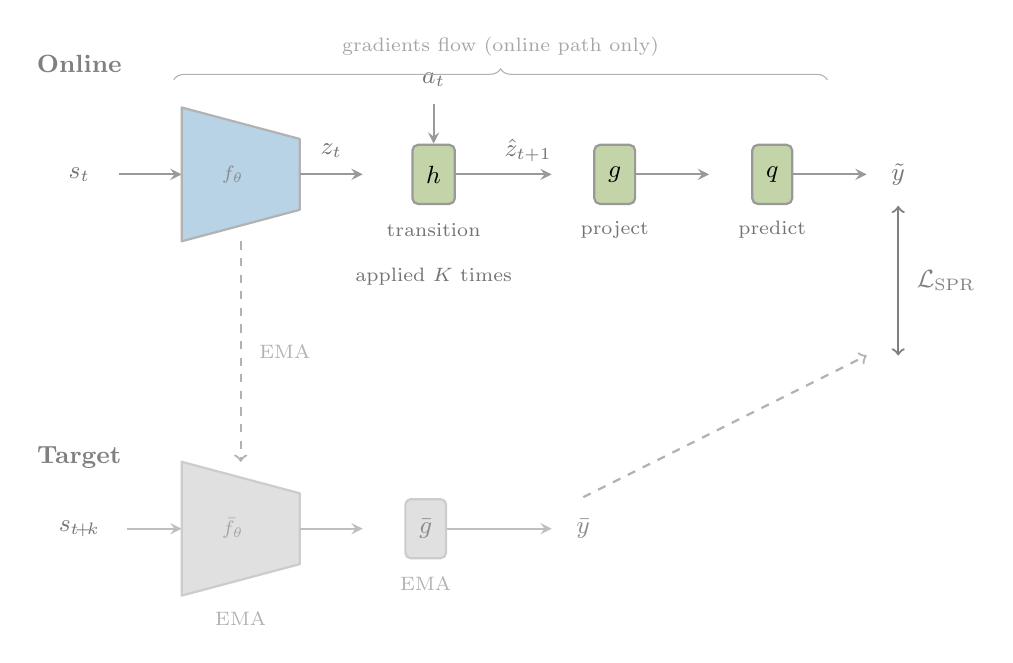
\begin{tikzpicture}[
    box/.style={draw=black!40, thick, minimum height=0.75cm,
                font=\small, inner sep=5pt, rounded corners=2pt},
    arr/.style={->, thick, >=stealth, black!40},
    lbl/.style={font=\scriptsize, text=black!55},
    mathlbl/.style={font=\small, text=black!55},
]

% === ONLINE PATH (top) ===
\node[lbl, font=\small\bfseries, text=black!50] at (-0.5, 2.2)
    {Online};

% s_t
\node[mathlbl] at (-0.5, 0.8) {$s_t$};
\draw[arr] (0.0, 0.8) -- (0.8, 0.8);

% Encoder
\fill[encfade, draw=black!30, thick, line join=round]
    (0.8, -0.05) -- (0.8, 1.65) -- (2.3, 1.25) -- (2.3, 0.35) -- cycle;
\node[font=\scriptsize, text=black!45] at (1.45, 0.8) {$f_\theta$};

% z_t
\draw[arr] (2.3, 0.8) -- (3.1, 0.8);
\node[mathlbl] at (2.7, 1.1) {$z_t$};

% Transition model
\node[box, fill=sprcomp] (trans) at (4.0, 0.8) {$h$};
\node[lbl] at (4.0, 0.1) {transition};

% Action input
\node[mathlbl] at (4.0, 2.0) {$a_t$};
\draw[arr] (4.0, 1.7) -- (trans.north);

% z_hat_{t+1}
\draw[arr] (trans.east) -- (5.5, 0.8);
\node[mathlbl] at (5.2, 1.1) {$\hat{z}_{t+1}$};

% Repeated application note
\node[lbl, align=center] at (4.0, -0.5)
    {applied $K$ times};

% Projection
\node[box, fill=sprcomp] (proj) at (6.3, 0.8) {$g$};
\node[lbl] at (6.3, 0.1) {project};

% y_hat
\draw[arr] (proj.east) -- (7.5, 0.8);

% Prediction head
\node[box, fill=sprcomp] (pred) at (8.3, 0.8) {$q$};
\node[lbl] at (8.3, 0.1) {predict};

% pred output
\draw[arr] (pred.east) -- (9.5, 0.8);
\node[mathlbl] at (9.9, 0.8) {$\tilde{y}$};

% === TARGET PATH (bottom) ===
\node[lbl, font=\small\bfseries, text=black!50] at (-0.5, -2.8)
    {Target};

% s_{t+k}
\node[mathlbl] at (-0.5, -3.7) {$s_{t\!+\!k}$};
\draw[arr, black!25] (0.1, -3.7) -- (0.8, -3.7);

% EMA Encoder
\fill[targetfade, draw=black!20, thick, line join=round]
    (0.8, -4.55) -- (0.8, -2.85) -- (2.3, -3.25) -- (2.3, -4.15) -- cycle;
\node[font=\scriptsize, text=black!35] at (1.45, -3.7) {$\bar{f}_\theta$};
\node[lbl, text=black!30] at (1.55, -4.85) {EMA};

% z_tilde
\draw[arr, black!25] (2.3, -3.7) -- (3.1, -3.7);

% EMA Projection
\node[box, fill=targetfade, draw=black!20, text=black!45]
    (tproj) at (3.9, -3.7) {$\bar{g}$};
\node[lbl, text=black!30] at (3.9, -4.4) {EMA};

% target output
\draw[arr, black!25] (tproj.east) -- (5.5, -3.7);
\node[mathlbl, text=black!45] at (5.9, -3.7) {$\bar{y}$};

% === EMA UPDATE ARROW ===
\draw[->, thick, dashed, black!30]
    (1.55, -0.05) -- (1.55, -2.85)
    node[midway, right=3pt, lbl, text=black!30] {EMA};

% === COSINE SIMILARITY ===
\draw[<->, thick, black!50]
    (9.9, 0.4) -- (9.9, -1.5)
    node[midway, right=3pt, font=\small, text=black!50]
    {$\mathcal{L}_{\mathrm{SPR}}$};

% Connect target output to loss
\draw[->, thick, dashed, black!30]
    (5.9, -3.3) -- (9.5, -1.5);

% Gradient annotation
\draw[decorate, decoration={brace, amplitude=4pt}, black!30]
    (0.7, 2.0) -- (9.0, 2.0)
    node[midway, above=5pt, lbl, text=black!35]
    {gradients flow (online path only)};

\end{tikzpicture}
\caption{SPR training architecture. The online encoder $f_\theta$
  produces spatial features $z_t$, which the transition model $h$
  rolls forward $K$ steps using actions. Projected predictions are
  compared via cosine similarity to targets from the EMA encoder
  $\bar{f}_\theta$. The prediction head $q$ exists only on the
  online side, creating the asymmetry that prevents representation
  collapse. Gradients flow through the online path only; the target
  network is updated via exponential moving average.}
\label{fig:spr-architecture}
\end{figure}
